\documentclass{qazcho_tasks}
\usepackage[utf8]{inputenc}

\ProvidesFile{siunitx.cfg} 
% Put any \sisetup{} command here too

% Основные единицы (SI base units, Table 1)

% Наименование                  Символ размерности Русское наименование Французское наименование Английское наименование Русское обозначение Международное обозначение
% Длина                         L                  метр                 mètre                    metre                   м                   m
% Масса                         M                  килограмм            kilogramme               kilogram                кг                  kg
% Время                         T                  секунда              seconde                  second                  с                   s
% Сила электрического тока      I                  ампер                ampère                   ampere                  А                   A
% Термодинамическая температура Θ                  кельвин              kelvin                   kelvin                  К                   K
% Количество вещества           N                  моль                 mole                     mole                    моль                mol
% Сила света                    J                  кандела              candela                  candela                 кд                  cd

\DeclareSIUnit\metre{\text{м}}
\DeclareSIUnit\meter{\text{м}}
%\DeclareSIUnit\kilogram{\text{кг}} % определяется через грамм
\DeclareSIUnit\second{\text{с}}
\DeclareSIUnit\ampere{\text{А}}
\DeclareSIUnit\kelvin{\text{К}}
\DeclareSIUnit\mole{\text{моль}}
\DeclareSIUnit\candela{\text{кд}}


% Производные единицы, имеющие специальные наименования и обозначения (Coherent derived units in the SI with special names and symbols, Table 2)

% Величина                                 Русское наименование Английское наименование Русское обозначение Международное обозначение Выражение через основные единицы
% Активность радиоактивного источника      беккерель            becquerel               Бк                  Bq                        с−1
% Температура Цельсия                      градус Цельсия       degree Celsius          °C                  °C                        K
% Электрический заряд                      кулон                coulomb                 Кл                  C                         А·с
% Электроёмкость                           фарад                farad                   Ф                   F                         Кл/В=с4·А2·кг−1·м−2
% Масса                                    грамм                gram                    г                   g                         10-3кг
% Поглощённая доза ионизирующего излучения грей                 gray                    Гр                  Gy                        Дж/кг=м²/c²
% Частота                                  герц                 hertz                   Гц                  Hz                        с−1
% Индуктивность                            генри                henry                   Гн                  H                         кг·м2·с−2·А−2
% Энергия                                  джоуль               joule                   Дж                  J                         Н·м=кг·м2·c−2
% Активность катализатора                  катал                katal                   кат                 kat                       моль/с
% Световой поток                           люмен                lumen                   лм                  lm                        кд·ср
% Освещённость                             люкс                 lux                     лк                  lx                        лм/м²=кд·ср/м²
% Сила                                     ньютон               newton                  Н                   N                         кг·м·c−2
% Сопротивление                            ом                   ohm                     Ом                  Ω                         В/А=кг·м2·с−3·А−2
% Давление                                 паскаль              pascal                  Па                  Pa                        Н/м2=кг·м−1·с−2
% Плоский угол                             радиан               radian                  рад                 rad                       м·м−1=1
% Электрическая проводимость               сименс               siemens                 См                  S                         Ом−1=с3·А2·кг−1·м−2
% Эффективная доза ионизирующего излучения зиверт               sievert                 Зв                  Sv                        Дж/кг=м²/c²
% Телесный угол                            стерадиан            steradian               ср                  sr                        м2·м−2=1
% Магнитная индукция                       тесла                tesla                   Тл                  T                         Вб/м2=кг·с−2·А−1
% Разность потенциалов                     вольт                volt                    В                   V                         Дж/Кл=кг·м2·с−3·А−1
% Мощность                                 ватт                 watt                    Вт                  W                         Дж/с=кг·м2·c−3
% Магнитный поток                          вебер                weber                   Вб                  Wb                        кг·м2·с−2·А−1

\DeclareSIUnit\becquerel{\text{Бк}}
%\DeclareSIUnit\degreeCelsius{\text{°C}}
\DeclareSIUnit\coulomb{\text{Кл}}
\DeclareSIUnit\farad{\text{Ф}}
\DeclareSIUnit\gram{\text{г}}
\DeclareSIUnit\gray{\text{Гр}}
\DeclareSIUnit\hertz{\text{Гц}}
\DeclareSIUnit\henry{\text{Гн}}
\DeclareSIUnit\joule{\text{Дж}}
\DeclareSIUnit\katal{\text{кат}}
\DeclareSIUnit\lumen{\text{лм}}
\DeclareSIUnit\lux{\text{лк}}
\DeclareSIUnit\newton{\text{Н}}
\DeclareSIUnit\ohm{\text{Ом}}
\DeclareSIUnit\pascal{\text{Па}}
\DeclareSIUnit\radian{\text{рад}}
\DeclareSIUnit\siemens{\text{См}}
\DeclareSIUnit\sievert{\text{Зв}}
\DeclareSIUnit\steradian{\text{ср}}
\DeclareSIUnit\tesla{\text{Тл}}
\DeclareSIUnit\volt{\text{В}}
\DeclareSIUnit\watt{\text{Вт}}
\DeclareSIUnit\weber{\text{Вб}}


% Единицы, не входящие в СИ (Non-SI units accepted for use with the International System of Units, Table 3)

% Единица         Английское наименование Русское обозначение Международное обозначение Величина в единицах СИ
% сутки           day                     сут                 d                         24ч=86400с
% угловой градус  degree                  °                   °                         (π/180)рад
% минута          minute                  мин                 min                       60с
% гектар          hectare                 га                  ha                        10000м²
% час             hour                    ч                   h                         60мин=3600с
% литр            litre                   л                   l,L                       0,001м³
% угловая минута  minute                  ′                   ′                         (1/60)°=(π/10800)
% угловая секунда second                  ″                   ″                         (1/60)′=(π/648000)
% тонна           tonne                   т                   t                         1000кг

\DeclareSIUnit\day{\text{сут}}
%\DeclareSIUnit\degree{\text{°}}
\DeclareSIUnit\hectare{\text{га}}
\DeclareSIUnit\hour{\text{ч}}
\DeclareSIUnit\litre{\text{л}}
\DeclareSIUnit\liter{\text{л}}
%\DeclareSIUnit\arcminute{\text{′}}
\DeclareSIUnit\minute{\text{мин}}
%\DeclareSIUnit\arcsecond{\text{″}}
\DeclareSIUnit\tonne{\text{т}}


% Non-SI units whose values in SI units must be obtained experimentally, Table 4

\DeclareSIUnit\astronomicalunit{\text{а. е.}}
\DeclareSIUnit\atomicmassunit{\text{а. е. м.}}
%\bohr
%\clight
\DeclareSIUnit\dalton{\text{а. е. м.}}
%\electronmass
\DeclareSIUnit\electronvolt{\text{эВ}}
%\elementarycharge
%\hartree
%\planckbar


% Other non-SI units, Table 5

% Единица      Английское наименование Русское обозначение Международное обозначение Величина в единицах СИ
% ангстрем     ångström                Å                   Å                         10−10м
% бар          bar                     бар                 bar                       100000 Па
% барн         barn                    б                   b                         10−28м²
% бел          bel                     Б                   B                         безразмерна
% узел         knot                    уз                  kn                        1 морская миля в час = (1852/3600) м/с
% морская миля nautical mile           миля                M                         1852 м (точно)
% непер        neper                   Нп                  Np                        безразмерна

%\DeclareSIUnit\angstrom{\text{Å}}
%\DeclareSIUnit\are{\text{а}} % ар (100 м²) не имеет макроса в siunitx по умолчанию
\DeclareSIUnit\bar{\text{бар}}
\DeclareSIUnit\barn{\text{б}}
\DeclareSIUnit\bel{\text{Б}}
\DeclareSIUnit\decibel{\text{дБ}}
\DeclareSIUnit\knot{\text{уз}}
\DeclareSIUnit\mmHg{\text{мм рт. ст.}}
\DeclareSIUnit\nauticalmile{\text{миля}}
\DeclareSIUnit\neper{\text{Нп}}


% SI prefixes, Table 6

% Степень Русская приставка Международная приставка Русское обозначение Международное обозначение
% 1       дека              deca                    да                  da
% 2       гекто             hecto                   г                   h
% 3       кило              kilo                    к                   k
% 6       мега              mega                    М                   M
% 9       гига              giga                    Г                   G
% 12      тера              tera                    Т                   T
% 15      пета              peta                    П                   P
% 18      экса              exa                     Э                   E
% 21      зетта             zetta                   З                   Z
% 24      иотта             yotta                   И                   Y

\DeclareSIPrefix\deca{\text{да}}{1} 
\DeclareSIPrefix\hecto{\text{г}}{2} 
\DeclareSIPrefix\kilo{\text{к}}{3}
\DeclareSIPrefix\mega{\text{М}}{6}
\DeclareSIPrefix\giga{\text{Г}}{9}
\DeclareSIPrefix\tera{\text{Т}}{12}
\DeclareSIPrefix\peta{\text{П}}{15}
\DeclareSIPrefix\exa{\text{Э}}{18}
\DeclareSIPrefix\zetta{\text{З}}{21}
\DeclareSIPrefix\yotta{\text{И}}{24}


% Степень Русская приставка Международная приставка Русское обозначение Международное обозначение
% -1      деци              deci                    д                   d
% -2      санти             centi                   с                   c
% -3      милли             milli                   м                   m
% -6      микро             micro                   мк                  µ
% -9      нано              nano                    н                   n
% -12     пико              pico                    п                   p
% -15     фемто             femto                   ф                   f
% -18     атто              atto                    а                   a
% -21     зепто             zepto                   з                   z
% -24     иокто             yocto                   и                   y

\DeclareSIPrefix\deci{\text{д}}{-1}
\DeclareSIPrefix\centi{\text{с}}{-2}
\DeclareSIPrefix\milli{\text{м}}{-3}
\DeclareSIPrefix\micro{\text{мк}}{-6}
\DeclareSIPrefix\nano{\text{н}}{-9}
\DeclareSIPrefix\pico{\text{п}}{-12}
\DeclareSIPrefix\femto{\text{ф}}{-15}
\DeclareSIPrefix\atto{\text{а}}{-18}
\DeclareSIPrefix\zepto{\text{з}}{-21}
\DeclareSIPrefix\yocto{\text{и}}{-24}


% Степень Международное обозначение Международная приставка Русское обозначение Русское написание числа бит Русская приставка
% 10      kibi                      Ki                      киби                Кибит                       Ки
% 20      mebi                      Mi                      меби                Мибит                       Ми
% 30      gibi                      Gi                      гиби                Гибит                       Ги
% 40      tebi                      Ti                      теби                Тибит                       Ти
% 50      pebi                      Pi                      пеби                Пибит                       Пи
% 60      exbi                      Ei                      эксби               Эибит                       Эи
% 70      zebi                      Zi                      зеби                Зибит                       Зи
% 80      yobi                      Yi                      йоби                Йибит                       Йи

\DeclareBinaryPrefix\kibi{\text{Ки}}{10}
\DeclareBinaryPrefix\mebi{\text{Ми}}{20}
\DeclareBinaryPrefix\gibi{\text{Ги}}{30}
\DeclareBinaryPrefix\tebi{\text{Ти}}{40}
\DeclareBinaryPrefix\pebi{\text{Пи}}{50}
\DeclareBinaryPrefix\exbi{\text{Эи}}{60}
\DeclareBinaryPrefix\zebi{\text{Зи}}{70}
\DeclareBinaryPrefix\yobi{\text{Йи}}{80}



% Положение о единицах величин, допускаемых к применению в Российской Федерации,
% разрешает применение следующих внесистемных единиц:
% карат
% град (гон)
% световой год
% парсек
% фут
% дюйм
% килограмм-сила на квадратный сантиметр
% миллиметр водяного столба
% метр водяного столба
% техническая атмосфера
% диоптрия
% текс
% гал
% оборот в секунду
% оборот в минуту
% киловатт-час
% вольт-ампер
% вар
% ампер-час
% бит
% байт
% бит в секунду
% байт в секунду
% рентген
% бэр
% рад
% рентген в секунду
% кюри
% стокс
% калория (международная)
% калория термохимическая
% калория 15-градусная
% калория в секунду
% килокалория в час
% гигакалория в час

% Положение разрешает применять единицы относительных и логарифмических величин, такие как:
% процент
% промилле
% миллионная доля
% децибел
% фон
% октава
% декада

% Допускается также применять единицы времени, получившие широкое распространение, например:
% неделя
% месяц
% год
% век
% тысячелетие

% Не применяются с кратными и дольными приставками СИ наименования и обозначения внесистемных единиц:
% массы
% времени
% плоского угла
% длины
% площади
% давления
% оптической силы
% линейной плотности
% скорости
% ускорения
% частоты вращения

\title{qazcho_tasks}
\author{}
\date{}

\begin{document}

\titlepage{Заключительный этап}{2021-2022}{10}{chem10-1-tasks}

\tableofcontents

\section*{\fontspec{PT Sans} Регламент олимпиады:}
\addcontentsline{toc}{section}{Регламент олимпиады}

Перед вами находится комплект задач республиканской олимпиады 2022 года по химии. \textbf{Внимательно} ознакомьтесь со всеми нижеперечисленными инструкциями и правилами. У вас есть \textbf{5 астрономических часов (300 минут)} на выполнение заданий олимпиады. Ваш результат – сумма баллов за каждую задачу, с учетом весов каждой из задач.

Вы можете решать задачи в черновике, однако, не забудьте перенести все решения на листы ответов. Проверяться будет \textbf{только то, что вы напишете внутри специально обозначенных квадратиков}. Черновики проверяться \textbf{не будут}. Учтите, что вам \textbf{не будет выделено} дополнительное время на перенос решений на бланки ответов.

Вам \textbf{разрешается} использовать графический или инженерный калькулятор.

Вам \textbf{запрещается} пользоваться любыми справочными материалами, учебниками или конспектами.

Вам \textbf{запрещается} пользоваться любыми устройствами связи, смартфонами, смарт-часами или любыми другими гаджетами, способными предоставлять информацию в текстовом, графическом и/или аудио формате, из внутренней памяти или загруженную с интернета.

Вам \textbf{запрещается} пользоваться любыми материалами, не входящими в данный комплект задач, в том числе периодической таблицей и таблицей растворимости. На \textbf{странице 3} предоставляем единую версию периодической таблицы.

Вам \textbf{запрещается} общаться с другими участниками олимпиады до конца тура. Не передавайте никакие материалы, в том числе канцелярские товары. Не используйте язык жестов для передачи какой-либо информации.

За нарушение любого из данных правил ваша работа будет \textbf{автоматически} оценена в \textbf{0 баллов}, а прокторы получат право вывести вас из аудитории.

На листах ответов пишите \textbf{четко} и \textbf{разборчиво}. Рекомендуется обвести финальные ответы карандашом. \textbf{Не забудьте указать единицы} измерения \textbf{(ответ без единиц измерения будет не засчитан)}. Соблюдайте правила использования числовых данных в арифметических операциях. Иными словами, помните про существование значащих цифр.

Если вы укажете только конечный результат решения без приведения соответствующих вычислений, то Вы получите \textbf{0} баллов, даже если ответ правильный.

Решения этой олимпиады будут опубликованы на сайте \href{https://qazcho.kz}{www.qazcho.kz}.

Рекомендации по подготовке к олимпиадам по химии есть на сайте \href{https://kazolymp.kz}{www.kazolymp.kz}.


\phantomsection
\addcontentsline{toc}{section}{Периодическая таблица}

\begin{tabularx}{\textwidth}{|Y|Y|Y|Y|Y|Y|Y|Y|Y|Y|Y|Y|Y|Y|Y|Y|Y|Y|}
  \cline{1-1}\cline{18-18}
  \small 1 & \multicolumn{15}{c}{} & {} & \small 18 \\
  \cline{1-2}\cline{13-18}
  % period 1
  \chemelement{1}{H}{1.008} & \small 2 & \multicolumn{9}{c}{} & {} & \small 13 & \small 14 & \small 15 & \small 16 & \small 17 & \chemelement{2}{He}{4.003} \\
  \cline{1-2}\cline{13-18}
  % period 2
  \chemelement{3}{Li}{6.94} & \chemelement{4}{Be}{9.01} & \multicolumn{9}{c}{} & {} & \chemelement{5}{B}{10.81} & \chemelement{6}{C}{12.01} & \chemelement{7}{N}{14.01} & \chemelement{8}{O}{16.00} & \chemelement{9}{F}{19.00} & \chemelement{10}{Ne}{20.18} \\
  \hline
  % period 3
  \chemelement{11}{Na}{22.99} & \chemelement{12}{Mg}{24.31} & \small 3 & \small 4 & \small 5 & \small 6 & \small 7 & \small 8 & \small 9 & \small 10 & \small 11 & \small 12 & \chemelement{13}{Al}{26.98} & \chemelement{14}{Si}{28.09} & \chemelement{15}{P}{30.97} & \chemelement{16}{S}{32.06} & \chemelement{17}{Cl}{35.45} & \chemelement{18}{Ar}{39.95} \\
  \hline
  % period 4
  \chemelement{19}{K}{39.10} & \chemelement{20}{Ca}{40.08} & \chemelement{21}{Sc}{44.96} & \chemelement{22}{Ti}{47.87} & \chemelement{23}{V}{50.94} & \chemelement{24}{Cr}{52.00} & \chemelement{25}{Mn}{54.94} & \chemelement{26}{Fe}{55.85} & \chemelement{27}{Co}{58.93} & \chemelement{28}{Ni}{58.69} & \chemelement{29}{Cu}{63.55} & \chemelement{30}{Zn}{65.38} & \chemelement{31}{Ga}{69.72} & \chemelement{32}{Ge}{72.63} & \chemelement{33}{As}{74.92} & \chemelement{34}{Se}{78.97} & \chemelement{35}{Br}{79.90} & \chemelement{36}{Kr}{83.80} \\
  \hline
  % period 5
  \chemelement{37}{Rb}{85.47} & \chemelement{38}{Sr}{87.62} & \chemelement{39}{Y}{88.91} & \chemelement{40}{Zr}{91.22} & \chemelement{41}{Nb}{92.91} & \chemelement{42}{Mo}{95.95} & \chemelement{43}{Tc}{-} & \chemelement{44}{Ru}{101.1} & \chemelement{45}{Rh}{102.9} & \chemelement{46}{Pd}{106.4} & \chemelement{47}{Ag}{107.9} & \chemelement{48}{Cd}{112.4} & \chemelement{49}{In}{114.8} & \chemelement{50}{Sn}{118.7} & \chemelement{51}{Sb}{121.8} & \chemelement{52}{Te}{127.6} & \chemelement{53}{I}{126.9} & \chemelement{54}{Xe}{131.3} \\
  \hline
  % period 6
  \chemelement{55}{Cs}{132.9} & \chemelement{56}{Ba}{137.3} & {\small 57-71} & \chemelement{72}{Hf}{178.5} & \chemelement{73}{Ta}{180.9} & \chemelement{74}{W}{183.8} & \chemelement{75}{Re}{186.2} & \chemelement{76}{Os}{190.2} & \chemelement{77}{Ir}{192.2} & \chemelement{78}{Pt}{195.1} & \chemelement{79}{Au}{197.0} & \chemelement{80}{Hg}{200.6} & \chemelement{81}{Tl}{204.4} & \chemelement{82}{Pb}{207.2} & \chemelement{83}{Bi}{209.0} & \chemelement{84}{Po}{-} & \chemelement{85}{At}{-} & \chemelement{86}{Rn}{-} \\
  \hline
  % period 7
  \chemelement{87}{Fr}{-} & \chemelement{88}{Ra}{-} & {\small 89-103} & \chemelement{104}{Rf}{-} & \chemelement{105}{Db}{-} & \chemelement{106}{Sg}{-} & \chemelement{107}{Bh}{-} & \chemelement{108}{Hs}{-} & \chemelement{109}{Mt}{-} & \chemelement{110}{Ds}{-} & \chemelement{111}{Rg}{-} & \chemelement{112}{Cn}{-} & \chemelement{113}{Nh}{-} & \chemelement{114}{Fl}{-} & \chemelement{115}{Mc}{-} & \chemelement{116}{Lv}{-} & \chemelement{117}{Ts}{-} & \chemelement{118}{Og}{-} \\
  \hline
  \multicolumn{18}{c}{} \\
  \cline{4-18}
  % period 8
  \multicolumn{2}{c}{} & {} & \chemelement{57}{La}{138.9} & \chemelement{58}{Ce}{140.1} & \chemelement{59}{Pr}{140.9} & \chemelement{60}{Nd}{144.2} & \chemelement{61}{Pm}{-} & \chemelement{62}{Sm}{150.4} & \chemelement{63}{Eu}{152.0} & \chemelement{64}{Gd}{157.3} & \chemelement{65}{Tb}{158.9} & \chemelement{66}{Dy}{162.5} & \chemelement{67}{Ho}{164.9} & \chemelement{68}{Er}{167.3} & \chemelement{69}{Tm}{168.9} & \chemelement{70}{Yb}{173.0} & \chemelement{71}{Lu}{175.0} \\
  \cline{4-18}
  % period 9
  \multicolumn{2}{c}{} & {} & \chemelement{89}{Ac}{-} & \chemelement{90}{Th}{232.0} & \chemelement{91}{Pa}{231.0} & \chemelement{92}{U}{238.0} & \chemelement{93}{Np}{-} & \chemelement{94}{Pu}{-} & \chemelement{95}{Am}{-} & \chemelement{96}{Cm}{-} & \chemelement{97}{Bk}{-} & \chemelement{98}{Cf}{-} & \chemelement{99}{Es}{-} & \chemelement{100}{Fm}{-} & \chemelement{101}{Md}{-} & \chemelement{102}{No}{-} & \chemelement{103}{Lr}{-} \\
   \cline{4-18}
\end{tabularx}


\problem{Химический блиц}{8}

\ProblemPointsSeven{2}{3}{3}{4}{4}{2}{3}{21}{8}

Предлагаем вам сделать небольшую интеллектуальную разминку и решить следующие задачи.

\begin{enumerate}
  \item Установите формулу оксида, в котором массовая доля кислорода равна 56.36\%.
  \item Запишите уравнения реакций разложения а) нитрата калия, б) нитрата цинка, в) нитрата серебра.
  \item Запишите уравнения реакций перманганата калия с нитритом калия в а) серной кислоте, б) воде, в) гидроксиде калия.
  \item На полное восстановление 7.57 г смеси оксидов железа (II) и меди потребовалось 2.24 л молекулярного водорода (при н. у.). Определите массовые доли оксидов в исходной смеси.
  \item ``Нужно больше олеума'' подумал химик. Какую массу 20\% (по массе) олеума необходимо добавить к 50 г 98\% (по массе) серной кислоты, чтобы получить олеум с массовой долей в 1.804\%?
  \item Запишите полную электронную конфигурацию атома меди.
  \item Определите степени оксиления каждого атома в следующих веществах: а) $\ce{K4[Fe(CN)6]}$, б) $\ce{Na2Cr2O7}$, в) $\ce{I2}$.
\end{enumerate}


\problem{В чем сила? (Моргунов А.)}{11}

\ProblemPointsFour{6}{8}{4}{5}{23}{11}


\begin{solbox}{6 баллов}
  Единственная информация, которая у нас есть о соединении \em{1} исходит от Антона, Дильназ и Малены, которые, судя по всему, говорят о хлоре, фторе и броме соответственно. Допустим Малена говорит правду. Тогда \em{1} – бром. Но Малена тут же говорит о том, что $\ce{Br2}$ вступает в реакцию с $\ce{NaCl}$ c образованием $\ce{Cl2}$. Такого быть не может – вытеснять галогены из галогенидов могут только более активные галогены, а бром менее активен чем хлор. Значит Малена – лжец (1 балл).

  Допустим Тания говорит правду – тогда \em{3} – это высший оксид. Но высший оксид, растворяясь в гидроксиде натрия, никак не может быть восстановителем – элемент уже находится в высшей степени окисления. Значит Тания – лжец (1 балл).

  Поймать последнего лжеца гораздо сложнее. Допустим Антон говорит правду. Тогда и по массовым долям \em{2} и по массовым долям \em{3} становится понятно, что речь идет о хроме. В нулевой степени окисления у хрома \em{6} электронов. Газ \em{6}, являющийся ядовитым по утверждению Антона, это $\ce{CO}$. Но $\ce{CO}$ – это лиганд сильного поля, значит соединение \em{5} обязано быть низкоспиновым. Но шесть электронов в низкоспиновой конфигурации никак не могут приводить к парамагнитным свойствам. Получаем противоречие. Значит Антон – лжец (2 балла)

  Таким образом, Богдан и Дильназ рыцари (2 балла)
\end{solbox}



\begin{solbox}{8 баллов}
  Определение элемента \em{X} можно провести и по соединению \em{2}, и по соединению \em{3}.

  Соединение \em{2} фторид, с общей формулой $\ce{EF_n}$

  \begin{gather*}
    \frac{x}{x + 19n} = 0.3490 \\
    2.865 x = x + 19n \\
    1.865 x = 19 n \\
    x = 10.188 n
  \end{gather*}

  Проверим разные варианты значений $n$

  \begin{tabularx}{\textwidth}{|X|X|X|X|X|X|X|X|}
    \hline
    n & 1 & 2 & 3 & 4 & 5 & 6 & 7 \\
    \hline
    x & 10.188 & 20.376 & 30.564 & 40.752 & 50.94 & 61.128 & 71.316 \\
    \hline
  \end{tabularx}

  С одной стороны можно подумать, что \em{X} — это фосфор, а \em{2} — это $\ce{PF3}$. Однако, массовая доля фосфора в $\ce{P2O5}$ всего лишь 43.6\%. Тогда \em{X} это ванадий (1 балл), \em{1} — это $\ce{F2}$ (1 балл), а \em{2} — это $\ce{VF5}$ (1 балл)

  Подтвердить ванадий можно и с помощью расчетов по \em{3}.
  
  Определим формулу соединения \em{3}. В общем виде оксиды имеют формулу $\ce{X_nO_m}$. Возьмем атомную массу \em{X} за $x$

  \begin{gather*}
    \frac{nx}{nx + 16m} = 0.5601 \\
    1.785 nx = nx + 16m \\
    0.785 nx = 16m \\
    x = 20.382 \frac{m}{n}
  \end{gather*}
\end{solbox}
  
\begin{emptysolbox}
  Рассмотрим разные значения для $m$ и $n$
  
  \begin{tabularx}{\textwidth}{|X|X|X|X|X|X|X|X|X|}
    \hline
    n & 1 & 1 & 1 & 1 & 2 & 2 & 2 & 2 \\
    \hline
    m & 1 & 2 & 3 & 4 & 1 & 3 & 5 & 7 \\
    \hline
    x & 20.382 & 40.764 & 61.146 & 81.528 & 10.191 & 30.573 & 50.955 & 71.337 \\
    \hline
  \end{tabularx}

  Единственный подходящий вариант — комбинация $n = 2$ и $m = 5$, соответствующая элементу Ванадий (V).

  Таким образом \em{3} – $\ce{V2O5}$ (1 балл)

  Соединением \em{4} является соль натрия, которая может иметь формулу $\ce{NaVO3}$ или $\ce{Na3VO4}$ (проводя параллели с другими анионами с элементами в степени окисления +5). Проверки массовых долей подтверждают второй вариант: соединение \em{3} – это $\ce{Na3VO4}$ (1 балл)

  Наконец, основной компонент воздуха с молекулярной массой 28~\unit{\gmol} (соединение \em{6}) это азот $\ce{N2}$ (1 балл)

  Формула \em{5} необычна, но подтверждается массовыми долями: это [$\ce{V(N2)6}$] (2 балла). Справка: это соединение было выделено при 20-25~\unit{\kelvin} совместной конденсацией атомов ванадия и молекул азота.
\end{emptysolbox}



\begin{solbox}{4 балла}
  \begin{equation*}
    \ce{V + \frac{5}{2} F2 -> VF5}
  \end{equation*}

  (1 балл – образование \em{2})

  \begin{equation*}
    \ce{2VF5 <=> [VF4]+ + [VF6]-}
  \end{equation*}

  (1 балл – уравнение автопротолиза)

  Растворение оксида в гидроксиде натрия (1 балл):

  \begin{equation*}
    \ce{V2O5 + 6NaOH -> 2Na3VO4 + 3H2O}
  \end{equation*}

  Пентаоксид диванадия катализирует реакцию окисления диоксида серы (1 балл)

  \begin{equation*}
    \ce{SO2 + \frac{1}{2} O2 -> SO3}
  \end{equation*}
\end{solbox}



\begin{solbox}{3 балла}
  Санжар рыцарь (1 балл)

  Допустим в соединении \em{7} один атом ванадия. Тогда на остальные атомы приходится:

  \begin{equation*}
    \frac{50.94}{0.3514} \cdot 0.6486 = 94~\unit{\gmol}
  \end{equation*}

  Очевидно среди них есть атомы азота и кислорода, причем на каждый атом азота как минимум 3 атома кислорода. Нитратная группировка имеет массу 62~\unit{\gmol}. Остаток в 32~\unit{\gmol} может соответствовать еще двум атомам кислорода, что  соответствует форме ванадия в степени окисления +5 в кислой среде в виде диоксованадия. 

  Итого формула \em{7} - $\ce{VO2NO3}$ (2 балла). 0 баллов если в предлагаемой формуле нет катиона $\ce{VO2+}$.

  Проводя аналогичные рассуждения с \em{8}, на один атом ванадия приходится 112~\unit{\gmol} других элементов, из которых 96~\unit{\gmol} занимает сульфат. Таким образом \em{8} это сульфат ванадила:

  $\ce{VOSO4}$ (2 балла). 0 баллов если в предлагаемой формуле нет катиона $\ce{VO^2+}$
\end{solbox}


\problem{Масс-спектрометрия в органической химии}{8}

\ProblemPointsTwo{6}{4}{10}{8}

\hfill
\begin{minipage}{0.5\textwidth}
  \raggedleft
  Теория становится материальной силой, как только она овладевает массами.

  \textit{Карл Маркс.}\\
  \textit{К критике гегелевской философии права}
\end{minipage}

Суть масс-спектрометрического анализа заключается в переводе молекул образца в ионизированную форму с последующим разделением и регистрацией образующихся при этом положительных или отрицательных ионов.

Одним из важнейших преобразований ионов является перегруппировка
Мак-Лафферти. Она протекает благодаря миграции атома водорода
от $\gamma$-атома углерода через шестичленное переходное состояние:
\nopagebreak
\begin{figure}[H]
  \centering
  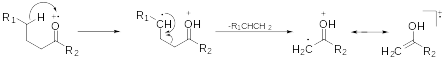
\includegraphics[width=0.9\textwidth]{problems/problem3/images/image1}
\end{figure}

\begin{enumerate}
  \item Для каких соединений произойдет перегруппировка Мак-Лафферти и для каких она будет подавлена? Ответ предоставьте схематически. Считайте, что катион-радикальный центр расположен на атоме кислорода.
  \nopagebreak
    \begin{enumerate}
      \item пентаналь
      \item гептен-5-он-2
      \item бутанон-2
      \item деканон-4
      \item октен-4-он-3
    \end{enumerate}

  \item Какому из изомерных соединений (пентаналь или 2-метилбутаналь) принадлежит указанный масс-спектр электронной ионизации? Ответ обоснуйте.
\end{enumerate}

\begin{minipage}{\textwidth}
  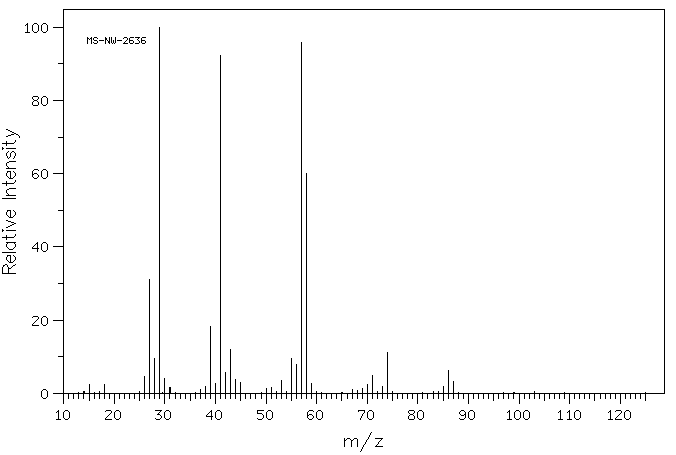
\includegraphics[width=0.65\textwidth]{problems/problem3/images/image2}
  \hspace{0.05\textwidth}
  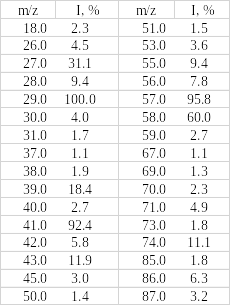
\includegraphics[width=0.3\textwidth]{problems/problem3/images/image3}
\end{minipage}


\problem{Кристаллохимия}{10}

\ProblemPointsSeven{4}{4}{6}{4}{4}{10}{8}{40}{10}

При взаимодействии металла \em{А} с неметаллом \em{Б} можно получить вещества \em{В} или \em{Г}, которые могут применяться как полупроводники и вещества, поглощающие микроволновое излучение.

Также синтез можно провести в гидротермальном реакторе при температурах выше 100\unit{\celsius}. Для этого смешивают водный раствор вещества \em{Д} с раствором, полученным растворением \em{Б} в растворе $\ce{NaOH}$ (\em{реакция 1}), затем добавляют к смеси гидразин ($\ce{N2H4}$) и нагревают в закрытой бомбе. В этой смеси при температурах 100-120\unit{\celsius} образуется чистый \em{Г} (\em{реакция 2}), а при температуре 180\unit{\celsius} через 6 часов кипячения образуется чистый \em{В} (\em{реакция 3}). \em{Реакции 2} и \em{3} протекают сложно: в них гидразин играет роль восстановителя, один из продуктов \em{реакции 1} --- роль окислителя, а \em{Д} --- источник металла \em{А}. Известен массовый состав вещества \em{Д}.

\begin{table}[H]
  \centering
  \begin{tabularx}{0.8\textwidth}{|Y|Y|Y|Y|}
    \hline
    $\omega (\mathbf{A})$ & $\omega (\mathbf{C})$ & $\omega (\mathbf{O})$ & $\omega (\mathbf{H})$ \\
    \hline
    26.28\% & 22.98\% & 45.92\% & 4.82\% \\
    \hline
  \end{tabularx}
\end{table}

На рисунках 1 и 2.\textit{а} показаны элементарные ячейки кристаллических решеток \em{В} и \em{Г}, соответственно. На рисунке 2.\textit{б} показан также вид сверху, совпадающий с видом спереди и сбоку, на ячейку \em{Г}. Сиреневые атомы --- \em{А}, оранжевые --- \em{Б}.

\begin{figure}[H]
  \centering
  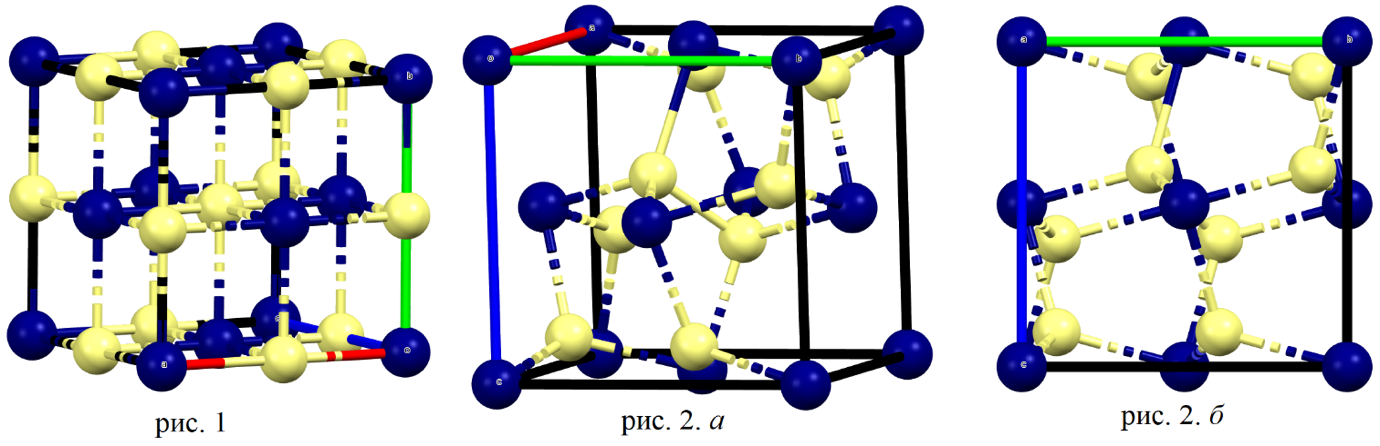
\includegraphics[width=\textwidth]{problems/problem4/images/image1}
\end{figure}

\begin{enumerate}
  \item Сколько атомов \em{А} и атомов \em{Б} расположено в одной элементарной ячейке вещества \em{В}? вещества \em{Г}?
  \item Каково координационное число \em{А} в веществе \em{В}? в веществе \em{Г}?
  \item Используя плотности и параметр ячеек \em{В} и \em{Г}, определите молярные массы элементов \em{А} и \em{Б}, запишите формулы \em{В} и \em{Г} и укажите степени окисления элементов в них.

  \begin{table}[H]
    \centering
    \begin{tabularx}{0.7\textwidth}{|Y|Y|Y|}
      \hline
       & $a,$ \unit{\angstrom} & $\rho,$ \unit{\gram\per\centi\meter\cubed} \\
      \hline
      \em{В} & 5.440 & 5.52 \\
      \hline
      \em{Г} & 6.417 & 5.35 \\
      \hline
    \end{tabularx}
  \end{table}

  \item Какова электронная конфигурация металла \em{А} в \em{В}? Приведите пример еще одного элемента в устойчивой степени окисления с такой же электронной конфигурацией.

  \item Приведите пример хотя бы одного природного вещества, изоструктурного \em{В}, и хотя бы одного природного вещества, изоструктурного \em{Г}.

  \item Определите формулу вещества \em{Д} и напишите уравнения \em{реакций 1--3}.
\end{enumerate}

\begin{minipage}{\textwidth}
  \begin{minipage}{0.6\textwidth}
    \begin{enumerate}
      \setcounter{enumi}{6}
      \item Подробное рассмотрение структуры \em{Г} показывает, что 2 атома \em{Б} (на рис. 3 помечены \textit{a} и \textit{b}) расположены на диагонали куба и равноудалены от вершин куба, образующих её концы. Известно, что расстояние от атома $a$ до ближайшего атома элемента \em{А} (помечен \textit{с}) составляет 2.379\unit{\angstrom}, а угол \textit{dac} при атоме a равен 75.8\unit{\degree}.

      Рассчитайте длину связи \em{Б-Б} (то есть расстояние \textit{ab}) в веществе \em{Г}.
    \end{enumerate}
  \end{minipage}
  \hspace{0.05\textwidth}
  \begin{minipage}{0.3\textwidth}
    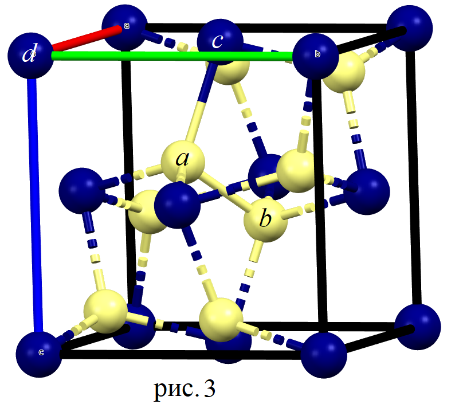
\includegraphics[width=\textwidth]{problems/problem4/images/image2}
  \end{minipage}
\end{minipage}

\problem{Учимся понимать кинетику}{11}

\begin{table}[H]
    \small
    \begin{tabularx}{\textwidth}{|X|X|X|X|X|X|X|X|X|X|X|}
        \hline
        \cellcolor{gray!45} \textbf{\arabic{problemcount}.1.1} & \cellcolor{gray!45} \textbf{\arabic{problemcount}.1.2} & \cellcolor{gray!45} \textbf{\arabic{problemcount}.1.3} & \cellcolor{gray!45} \textbf{\arabic{problemcount}.1.4} & \cellcolor{gray!45} \textbf{\arabic{problemcount}.2.1} & \cellcolor{gray!45} \textbf{\arabic{problemcount}.2.2} & \cellcolor{gray!45} \textbf{\arabic{problemcount}.2.3} & \cellcolor{gray!45} \textbf{\arabic{problemcount}.2.4} & \cellcolor{gray!45} \textbf{\arabic{problemcount}.2.5} & \cellcolor{gray!45} \textbf{Всего} & \cellcolor{gray!45} \textbf{Вес(\%)} \\
        \hline
        2 & 6 & 3 & 3 & 2 & 3 & 5 & 4 & 4 & 32 & 11 \\
        \hline
    \end{tabularx}
\end{table}

\subproblem{Подзадача 1. Реакция второго порядка.}

Однозначно, многие из Вас знакомы с различными порядками реакций. Для элементарных реакций (тех, в механизме которых замешана лишь одна стадия и отсутствуют вещества отличные от самих реагентов) скорость реакции пропорциональна концентрации реагирующих веществ.

Допустим, для реакции первого порядка:

\begin{gather}
    \notag \ce{A ->[k] \text{продукты}} \\
    \label{eq:first-order-one-reag} v_1 = k \cdot [A] = - \frac{dA}{dt}
\end{gather}

\begin{enumerate}
    \item Выведите зависимость концентрации вещества А от времени, решив дифференциальное уравнение (\ref{eq:first-order-one-reag}).
\end{enumerate}

Давайте рассмотрим наипростейший пример для реакции второго порядка типа

\begin{equation*}
    \ce{A + B ->[k] \text{продукты}}
\end{equation*}

Тогда вывод кинетического уравнения будет выглядить следующим образом:

\begin{equation*}
    k \cdot [\ce{A}] \cdot [\ce{B}] = - \frac{d[\ce{A}]}{dt}
\end{equation*}

Рассмотрим случай, когда начальные концентрации $[\ce{A}]_0$ и $[\ce{B}]_0$ равны. Так как $[\ce{A}]_0 = [\ce{B}]_0$, а стехиометрические коэффициенты говорят о том, что они расходуются одинаково, мы можем сказать, что $[\ce{A}] = [\ce{B}]$ в любой момент времени.

Тогда:

\begin{gather*}
    k [\ce{A}]^2 = -\frac{d[\ce{A}]}{dt} \\
    -kdt = [\ce{A}]^{-2} d[\ce{A}] \\
    -k \int\limits_{0}^{t_1} dt = \int\limits_{[\ce{A}]_0}^{[\ce{A}]_1} [\ce{A}]^{-2} d [\ce{A}] \\
    \frac{1}{[\ce{A}]_1} = \frac{1}{[\ce{A}]_0} + kt_1
\end{gather*}

Вот мы и вывели уравнение для реакции второго порядка при равных концентрациях реагентов. А что, если концентрации не равны?

\begin{enumerate}
    \setcounter{enumi}{1}
    \item Выведите кинетическое уравнение для случая, когда $[\ce{A}]_0 \neq [\ce{B}]_0$, при этом не забывайте, что А и В расходуются с одинаковой скоростью из-за равных стехиометрических коэффициентов.

    \textit{Подсказки:} вам может пригодиться записать выражение для $[\ce{B}]$ через $[\ce{B}]_0$, $[\ce{A}]_0$, $[\ce{A}]$. Также, для решения дифференциального уравнения Вам пригодится метод неопределенных коэффициентов, при котором интеграл сложной дроби разбивается на интегралы более простых дробей. Иными словами, любую дробь слева можно разбить на сумму дробей справа:
    
    \begin{equation*}
        \frac{1}{(x-a)(x-b)} = \frac{A}{x-a} + \frac{B}{x-b}
    \end{equation*}

    \item Некоторый индикатор окрашивает раствор в красный цвет при концентрации вещества А равному 0.01\unit{\moll}. Через какое время с начала реакции раствор потеряет свою окраску, если смешали 0.50\unit{\moll} раствор А с 0.80\unit{\moll} раствором В? Константа скорости реакции 0.59\unit{\per\second}.
    
    \item Какой порядок реакции будет наблюдаться если $[\ce{A}]_0 \gg [\ce{B}]_0$ (при этом $[\ce{B}]_0 \gg 1$)?
\end{enumerate}

\subproblem{Подзадача 2. Применение квазистационарного приближения.}

Наверняка, многие из Вас знакомы с схемой ферментативного катализа «ключ-замок». Однако, это простейшая схема ферментативного катализа. В задание ниже мы рассмотрим неконкурентное ингибирование.

\begin{enumerate}
    \item В чем отличие конкурентного ингибирования от неконкурентного с точки зрения строения фермента?
\end{enumerate}

Схему неконкурентного ингибирования можно записать следующим образом:

\begin{gather*}
    \ce{E + S <=>[k_1][k_{-1}] ES ->[k_2] E + P} \\
    \ce{E + I <=>[K_I] EI}
\end{gather*}

\begin{enumerate}
    \setcounter{enumi}{1}
    \item При каком соотношении констант возможно написать квазистационарное приближение для фермент-субстратного комплекса?
    
    \item Используя квазистационарное приближение для фермент-субстратного комплекса и уравнение материального баланса для всех форм фермента, выведите кинетическое уравнение. Напомним, что $\displaystyle K_M = \frac{k_{-1} + k_2}{k_1}$
\end{enumerate}

Фермент CYP2C9 участвует в катализе окисления ксенобиотиков – веществ, чужеродных для организма. Например, чтобы пометить ненасыщенные жирные кислоты для взаимодействия с другими ферментами, CYP2C9 катализирует реакцию эпоксидирования.

\begin{enumerate}
    \setcounter{enumi}{3}
    \item Запишите продукты реакции взаимодействия линолевой кислоты (цис,цис-9,12-октадекадиеновая кислота) с CYP2C9. Продуктом не может являться соединение, содержащие сразу две эпоксидные группы.
    
    \item Ингибиторами фермента CYP2C9 являются нифедипин, транилципропин, фенилизотиоцианат, и др. Они принимаются внутрь, чтобы снизить метаболическую активность ферментов против конкретных медицинских препаратов. Сравните скорость реакции эпоксидации при концентрациях ингибитора в крови $[\ce{I}] = 0$ и $[\ce{I}] = 0.5\unit{\moll}$, если
    концентрация субстрата в конкретный момент времени 0.183\unit{\moll}, а концентрация всех форм фермента 6\unit{\milli\moll}.
    
    Данные: $k_1 = 0.0042~\unit{\lmols}; \ k_{-1} = 0.00019~\unit{\per\second}; \ k_2 = 0.089~\unit{\per\second}; \ K_I = 1.89$
\end{enumerate}

\end{document}
